% $  Id: collabide.tex  $
% !TEX root = main.tex

%%
\section{CollabIDE}
\label{sec:collab-ide}

CollabIDE is a cloud-based integrated development environment presenting collaboration facilities 
distributed development teams working on a software project. CollabIDE has three key features which 
help to reduce the overhead of managing versions or product variants. These features are:
\begin{enumerate*}[label=(\arabic*)] 
\item version management, 
\item product variant management, and 
\item concurrent development.
\end{enumerate*}

%%
\subsection{Version Management}
Software products evolve over time~\cite{lehman02}. Rather than releasing a fully working product at once, developers implement products incrementally. Each product increment focuses on a single feature or part of the functionality at a time. Each of these features marks a new \emph{version} of the system, moving forward linearly in time. Defining and synchronizing between these pieces of functionality must be carried out multiple times in a project's lifespan. In the long-term, this process has a lasting impact in the productivity.

CollabIDE takes the association between a feature's development, and an associated version to that 
new feature to an extreme. In CollabIDE, every code modification (regardless of its size) is marked as 
a new product increment.
Furthermore, instead of asking developers to continuously create and manage product versions, 
CollabIDE automatically generates versions for each code increment. These increments are identified 
by a set of variables relevant to the project development and knowhow transfer. For example of all the  
available information from these versions take into account the name of the user creating the code 
increment, or the time of the day.
\fref{fig:versions} shows the way product versions are managed in the CollabIDE. 

Thanks to the concurrent development feature, all the team members obtain a new version the moment it is created. The developers can also switch between versions and view immediately the contents of the editor at the time the version was created or edited. 
As the time required for managing different product versions is reduced with this feature, this long-term impact can be reduced effectively.

\begin{figure}[htbp]
  \centering
  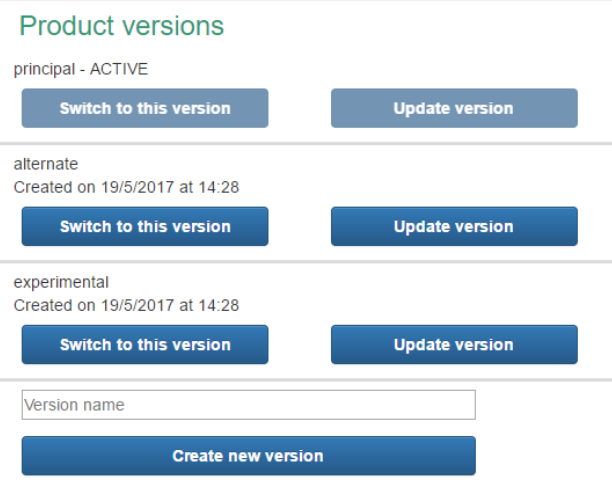
\includegraphics[width=0.7\textwidth]{img/fig4-collabIDEVersionManagement}
  \caption{Version visualization in CollabIDE}
  \label{fig:versions}
\end{figure}


%%
\subsection{Product Variant Management}
In a project, each developer is assigned a unique color which is used to highlight the contributions of code said developer has done. Additionally, each developer has a contribution state that determines if his contributions are visible or not to the rest of the team. In \fref{fig:} we show how this feature is integrated into the IDE. With contribution management, any developer can easily identify the contributions of each team member and toggle their visibility as needed. From a product variant point of view, this feature eases the process of building new variants from existing fragments of code, effectively reducing the overhead derived from executing initial configuration processes.

\begin{figure}[htbp]
  \centering
  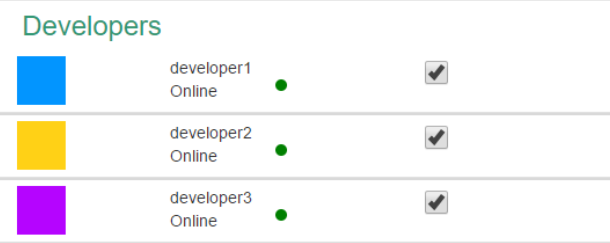
\includegraphics[width=0.7\textwidth]{img/fig3-collabIDEContributionManagement}
  \caption{}
  \label{fig:}
\end{figure}


%%
\subsection{Concurrent Development}
Using CollabIDE, developers are able to work concurrently on the same code base offering immediate feedback about the contributions of other developers.
Concurrent development means that all the actions a developer does in the IDE are synchronized. This lets all developers view in real time what changes are being made by other team members in the code editor or the control panel. In \fref{fig:} we show how the IDE highlights the code belonging to a certain team member. This feature eliminates the need of constantly having to obtain the latest changes made by other team members. Additionally, conflicts become nonexistent as there will always be only one version of the content being seen by the developers at a given time. The awareness of what each team member has done increases too with this feature, boosting coordination and allowing developers to know in little time what progress has been made in a project since the last time they worked on it. 

\begin{figure}[htbp]
  \centering
  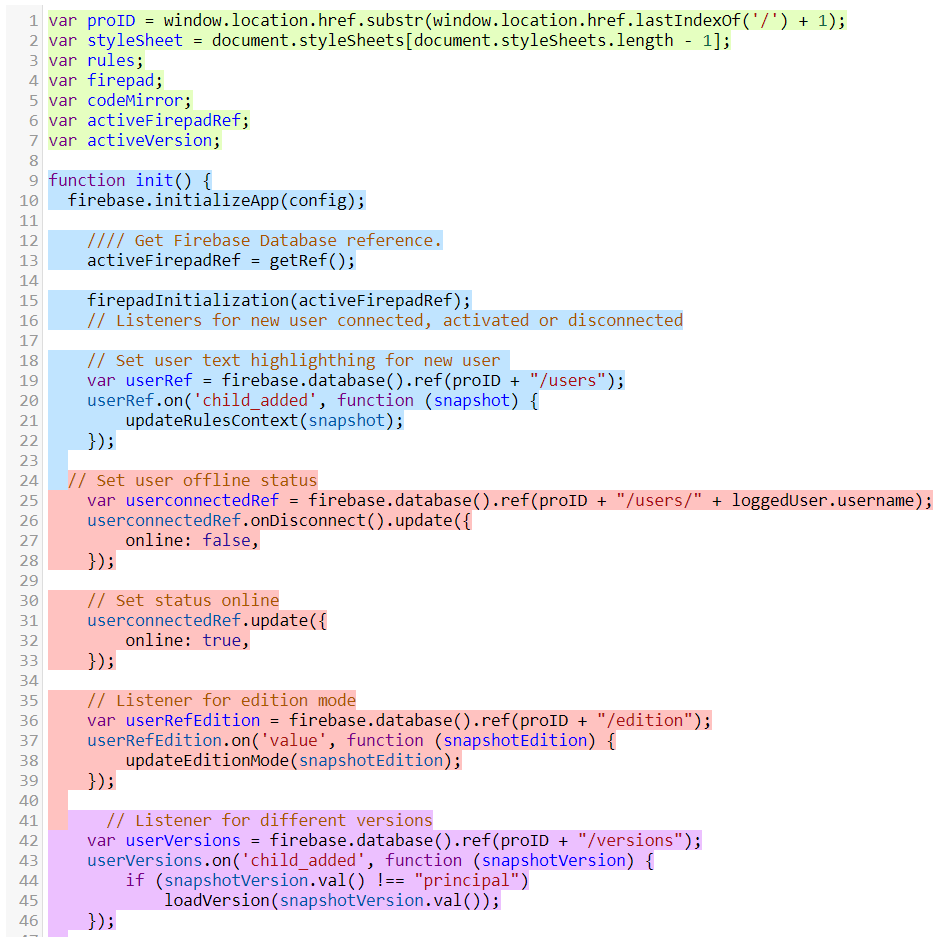
\includegraphics[width=0.7\textwidth]{img/fig2-collabIDEConcurrentProgramming}
  \caption{}
  \label{fig:}
\end{figure}


%%
\subsection{Implementation}
\label{sec:implementation}

The implementation of CollabIDE reconciles \ac{COP} with developing software systems integrated as part of a cloud-based platform.

%%%%
\subsubsection{\ac{COP} in a Nutshell}
The base of CollabIDE is \acf{COP}. \ac{COP} is a programming paradigm designed for the dynamic adaptation of software systems based on context information gathered from the system's surrounding execution environment~\cite{salvaneschi+12survey}. \ac{COP} consists of three main abstractions: \emph{Contexts}, \emph{Behavioral adaptations}, \emph{Adaptation activation}.

\paragraph{Contexts} represent semantically meaningful situations gathered from the systems surrounding environment~\cite{dey01}. Contexts are defined as first-class entities .

\paragraph{Behavioral adaptations,} are fine-grained behavior definitions associated to one or several context entities. Behavioral adaptations dictate the observable behavior of a system under particular situation sensed from the environment. The combination of behavioral adaptations and contexts constitute what we call and \emph{adaptation}.

\paragraph{Adaptations activation,} and their different combinations, are visible in the system through the activation and deactivation of context entities, effectively incorporating and withdrawing the behavioral adaptations associated with such contexts.


%%%%
\subsubsection{CollabIDE Internals}
To implement the features described previously, various contexts must be considered. Each developer 
and each product version represents a different context. To achieve this context management, we used 
the \ac{COP}, specifically using the Context Traits implementation~\cite{gonzalez13}. 
Context Traits provides the necessary elements to define a specific behavior during runtime for each 
context. CollabIDE features were build making use of these elements, which helped define the 
contribution state of a developer among other elements.
For the code editor of CollabIDE we used Firepad\footnote{\url{https://firepad.io/\#1}} which is an open 
source collaborative text editor. Firepad stores all the changes made in the editor in Firebase’s real 
time non relational database. Additional to the data Firepad stores, we store user and product versions 
data in Firebase.

\endinput
